\documentclass{template/custombook}
\usepackage{minted}
\usepackage{tikz}
\author{Dinal Atapattu}
\unitcoordinator{Dr. Matthew McKague}
\unitcode{CAB203}
\unitname{Discrete Structures}

\begin{document}
    \maketitle
    \tableofcontents
    \chapter{Tournament structure}
        The tournament structure is defined by two constraints:
            \begin{itemize}
                \item For every pair of distinct players, either they play against each other, or 
                there are at least two other players that they both play against
                \item All players have the same number of games
            \end{itemize}
        By abstracting the tournament to a graph structure, the players to vertices and the games to edges, these constraints can
        be represented as follows:
            \begin{flalign}
                \text{Constraint 1:} & \forall u,v \in V (u,v) \in E \wedge \left| N(u) \cap N(v)\right| \geq 2\\
                \text{Constraint 2:} & \forall v \in V \left| \text{deg}(v) \right| = 1
            \end{flalign}
        Where $V$ is the set of vertices, $E$ is the set of edges, $N(u)$ is the set of neighbours of $u$ and $\text{deg}(v)$ is the degree of $v$.
        Given the condition that a game between a and b is the same as a game between b and a, the given graph was symmetrised in order 
        to simplify the implementation. The symmetrisation was implemented as follows:
        \begin{flalign}
            \text{Symmetrisation:} & \forall u,v \in V (u,v) \in E \rightarrow (v,u) \in E
        \end{flalign}
        % This was implemented in Python as seen below
        % \inputminted[firstline=100, lastline=112]{python}{project.py}
        % The final solution was implemented as follows
        % \inputminted[firstline=6, lastline=24]{python}{project.py}
    \chapter{Assign referees}
        All games must have a referee, but referees cannot have any biases for the game they
        are refereeing, i.e., the referee cannot be a player in the game, have any relation to the players in the game,
        or any conflicts of interest in the game. Furthermore, to minimise the burden on referees, they are required to at
        most be assigned to one game.\\
        \begin{flalign}
            r \in R : c(r) \cap G = \emptyset\\
            R = \bigcup_{g\in G} f(g)
        \end{flalign}
        Assigning referees to games as a bipartite graph
        \begin{figure}[H]
            \centering
            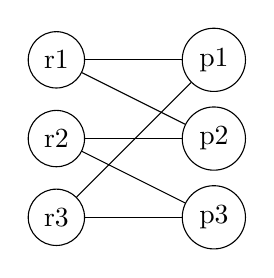
\begin{tikzpicture}
                \node[draw, circle] (r1) at (0,0) {r1};
                \node[draw, circle] (r2) at (0,-1) {r2};
                \node[draw, circle] (r3) at (0,-2) {r3};
                \node[draw, circle] (p1) at (2,0) {p1};
                \node[draw, circle] (p2) at (2,-1) {p2};
                \node[draw, circle] (p3) at (2,-2) {p3};
                \draw (r1) -- (p1);
                \draw (r1) -- (p2);
                \draw (r2) -- (p2);
                \draw (r2) -- (p3);
                \draw (r3) -- (p1);
                \draw (r3) -- (p3);
            \end{tikzpicture}
            \caption{Bipartite graph of referees and players}
        \end{figure}
    \chapter{Game groups}

    \chapter{Game schedule}

    \chapter{Tournament winners}
    
\end{document}